\documentclass[12pt]{article}
\usepackage{graphicx}
\usepackage[utf8]{inputenc}
\usepackage{makecell}
\usepackage[margin=0.7in]{geometry}
\usepackage[T1]{fontenc}
\usepackage{mathptmx}
\usepackage[normalem]{ulem}
\usepackage[section]{placeins}
 
\renewcommand\theadalign{bc}
\renewcommand\theadfont{\bfseries}
\renewcommand\theadgape{\Gape[4pt]}
\renewcommand\cellgape{\Gape[4pt]}

\usepackage[
backend=biber,
style=numeric,
sorting=none,
citestyle=ieee
]{biblatex}

\addbibresource{References.bib}

%opening
\title { \vspace{ Software Proposal Document for }
\newline Intelligent Surveillance for smart cities}
\author{Nour Ahmed , Mariam Hesham, Samiha Hesham, Sandra Fares}

\begin{document}

\begin{table}[htp]
\maketitle
\begin{tabular}{|l|l|l|}
\hline 
\thead{Proposal Version}    & \thead{Date} & \thead{Reason for Change}  \\ \hline
1.0 & 24-October-2020   & \makecell{Proposal First version’s specifications are defined}   \\ \hline 
2.0 & 26-October-2020   & \makecell{Similar systems, busniess applications added}   \\ \hline
\end{tabular}
\caption{Document version history}
\end{table}

\begin{table}[htp]
\begin{tabular}{cc}
\thead{GitHub:}    & {https://github.com/SandraFW/intelligent-Surveillance-for-smart-cities}   
\end{tabular}
\end{table}


\begin{abstract}
Surveillance systems are of vital importance for the development of smart cities. These systems can be considered vision organs of such cities. It is expected that a huge amount of data (Big Data) will be generated in smart cities. Therefore, to ensure the safety of its citizens, it is important to provide an efficient and real-time analysis of these data to get real-time responses, when catastrophic events occur. Accordingly, transmitting this massive data to the cloud, to be processed, is relatively slow. Therefore, the purpose of this project is to implement an edge computing- based surveillance system to offer real-time data processing. When surveillance videos capture an incident, the data get transferred to the edge for processing. Moreover, a rapid response is then provided to properly handle the occasion. Furthermore, despite tackling scalability obstacles, the system should handle privacy-sensitive data to overcome the privacy challenges in smart cities.
\end{abstract}
\newpage
\section{Introduction}

\subsection{Background}
The video surveillance system is a crucial component in the development of smart cities. Where it is useful for crime prevention, terrorist or forensic evidence detection, and traffic monitoring. However, the old traditional surveillance cannot accomplish these approaches, that's why smart surveillance systems with smart detection modules were introduced and always in enhancements till now.
 
However, implementing a citywide smart video surveillance system involves many challenges. A large number of cameras have to be deployed across the city, producing large amounts of data and information everyday. Besides, storing and enabling access to video devices and data at this large scale, in both real-time and on-demand manner, demand more computing and storage resources than traditional video surveillance systems. These challenges have to be addressed to maximize the effectiveness of smart video surveillance\cite{1}. 

Cloud computing was proposed then to solve some of those issues as mentioned in \cite{2} and \cite{3}, and it proved to be efficient but with the growth of data, it could not accomplish the desired results and the fast response due to the possible delay of transmitting the data to and from the cloud server. Moreover, it could not solve the privacy and security concerns. So, fog computing technology is recently introduced as a promising one to handle the current challenges of the surveillance systems development for smart cities.

\subsection{Motivation}
\subsubsection{Academic}
Since smart cities utilize IoT devices in recent times, in order to improve their infrastructure, numerous amounts of data get generated at a rapid rate. Passing data to the cloud is unfavorable when dealing with surveillance systems, as these systems require urgent and  instant responses to avoid misfortune events. Therefore, it is necessary to procure a strategy that will assist in managing and processing data effectively in a short period of time. Edge computing is a recently proposed solution for this problem. Instead of transferring data to the cloud, it gets transferred to the edge for real-time data processing. Various techniques are used to exploit this new technology and use it efficiently to solve different barriers. B. V. Natesha and Ram Mohana Reddy Guddeti \cite{nateshafog} proposed a fog computing based surveillance system, for smart cities, that processes data using deep learning methods in order to provide low latency and minimize the cost of the services. Likewise, G. Baldoni et al. \cite{baldoni2017dynamic} present edge computing to reduce the network traffic and offer scalability.
\subsubsection{Business}
With the expansion of IoT devices in smart cities, there is a massive amount of data generated from the cameras. The edge-based surveillance system provides businesses and organizations with significant benefits. It provides real-time data processing analysis, which helps the organizations to take proper action and make an immediate decision efficiently in case of accidents or abnormal events. Furthermore, huge organizations, like smart cities, need to keep their information and their citizens' data secure. Edge computing provides the system with security and privacy while working on lower bandwidth. Moreover, Edge computing needs limited storage to keep the data. So, there is no need for a central server for action-taking. Therefore, it provides the business and the organizations with lower costs.
\subsection{Problem Statement}
One of the challenges that face surveillance systems in smart cities is Big data, as the smart city involves huge amount of cameras in 24/7 mode to cover the whole city. Each camera records a massive amount of video and audio data to be processed. To handle such massive data, it is essential to provide a way to get real-time data processing analysis efficiently. Cloud computing has been utilized to perform data processing analysis, leading to slower performance. Therefore, edge computing is essential for real-time data processing analysis with high performance and low latency.


\section{Project Description}

\subsection{Objectives}
Our main objective is to build a fog computing based framework for surveillance data in order to detect abnormal human behaviors in the streets. We will improve an algorithm for anomaly detection  with remarkable stability and accuracy. The system is also developed to work on enhancing the latency by reducing the amount of data. Moreover, we will work on developing the privacy protection scheme for data security.
\begin{itemize}
\item The system will provide real time data processing analysis.

\item The system will response immediately and take a proper action when an event is detected.
\item The system will provide privacy assurance for the citizens.
\item The system will provide scalability with unlimited storage.
\end{itemize}

\subsection{Scope}
\begin{itemize}
\item Fog/Edge computing-based surveillance system to monitoring roads, streets, and squares in smart cities.
\item Scalability system to handle such massive data generated from surveillance cameras and sensors.
\item Efficiently detect any abnormal actions caused by human behavior and response immediately.
\item Privacy assurance by blur people's faces to secure their exposed identity in the video.

\end{itemize}
\newpage
\subsection{Project Overview}
\begin{figure}[!htbp]
  \centering
  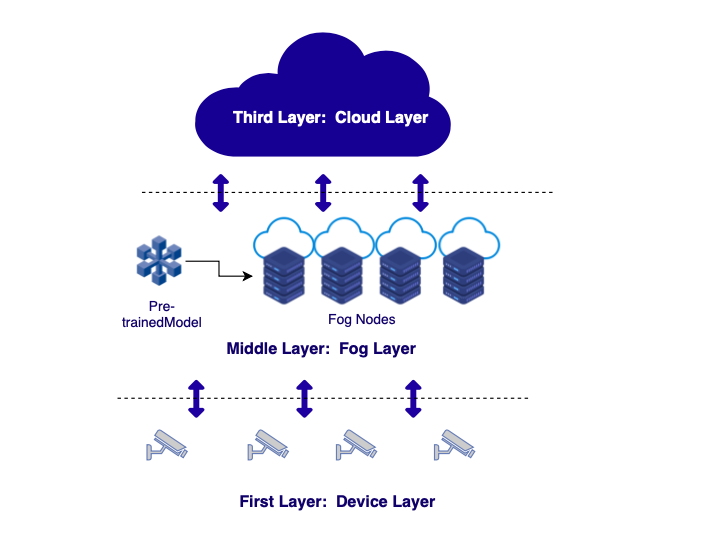
\includegraphics[width=10cm]{./1.png}
  \label{layers}
   \caption{three-layer fog computing architecture}
\end{figure}
Our system will be classified into three layers as shown in the figure. The first layer is the device layer where the surveillance cameras will capture the data and send those video streams over the network. Then, second, which is the fog layer, will do most of the work needed, as the videos will be processed on it using a pre-trained classification model for anomaly detection with the help of our fog nodes; this layer can also be divided into two layers in order to facilitate and reduce the overhead and after detection, if there's no abnormality in the streams, those streams will be summarized to reduce the huge amount of data that can be sent. Moreover, we will apply a securing algorithm to provide privacy while transferring the data, and send them to the cloud layer to be stored and retrieved easily.
\subsection{Stakeholder}
\subsubsection{Internal}

\begin{itemize}
\item Nour Ahmed (team leader)
\item Mariam Hesham
\item Sandra Fares
\item Samiha Hesham
\item Dr.Islam Tharwat
\item Eng.Lobna Shahen
\item Dr.Ashraf AbdelRaouf.
\end{itemize}


\subsubsection{External}
Ministry of communication, Elsewedy technology, Government companies, smart cities, and grand city shopping centers as they need our system to monitor their places 24/7 with unlimited storage.Also detecting any abnormal activity efficiently.

\section{Similar System}
\subsection{Academic}
\begin{itemize}
\item Jianyu Wang et al. \cite{wang2017elastic} designed fog computing architecture for urban surveillance systems to provide low latency and decrease the workload of cloud centers. The authors implemented Network Functions Virtualization and Software-Defined Networking on the cloud computing platform OpenStack, resulting in a real-time video processing system. Experimental results are promising. They show that the system can be developed on a larger scale and that fog computing can be potentially used for smart urban surveillance systems. 

\item In the hopes of exploiting fog computing and tackling the cost challenges faced when building surveillance systems, Mansoor Nasir et al \cite{nasir2019fog} presented a cost-effective fog computing based surveillance system. The system does not only reduce the energy consumed and the bandwidth, but also reduces the cost. The authors proposed a video summarization technique to reach their goal. By using Raspberry Pi devices as the system’s fog nodes, and by distributing data onto these nodes to provide a summary, the system is scalable and delivers satisfactory outcomes.

\item Ning Chen et al. \cite{chen2017smart} discussed in their chapter (Smart City Surveillance in Fog Computing) fog computing and its impact on smart city surveillance systems. Moreover, they stated the major challenges faced in smart cities, the advantages of fog computing compared to cloud computing, and introduced a traffic detection case study. The system architecture is made up of three layers demonstrated in Figure \ref{fog}: data collection, fog, and cloud center. In the system, drones capture video streams and send them to get processed, using target tracking and speed calculation algorithms, in the fog layer. Moreover, data can be transmitted to the cloud center for further long-term analysis. This approach provides real-time processing and covers a wide range of areas.
\begin{figure}[htp]
    \centering
    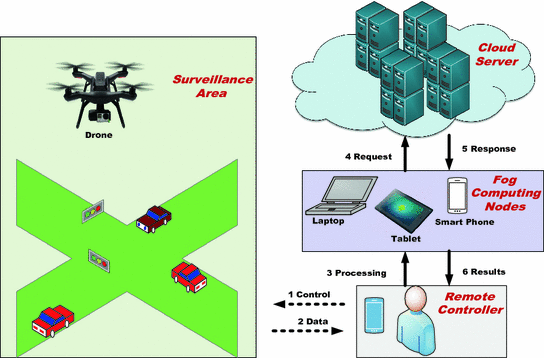
\includegraphics[width=10cm]{336804_1_En_9_Fig3_HTML.png}
    \caption{Fog-based Traffic Detection in Smart Cities}
    \label{fog}
\end{figure}
\newpage
\item Yutong Liu et al \cite{liu2019litedge} address the obstacles faced when working with wireless surveillance systems, since wireless systems improve the performance and are easier to manage. As the amount of data to be transmitted gets larger, the challenges become visible and the burden on the network increases. This system reduces the pressure on the network by filtering and applying video compression. Moreover, the system provides real-time processing and monitoring using edge computing approach. Experimental results show that the system accomplishes 82 percent latency reduction. As well as, 91.26 percent transmission workload reduction as the redundant data get filtered out.
\item Natesha et al \cite{nateshafog} proposed two fog architecture as an experiment to reduce latency and cloud resource consumption. The first architecture, shown in Figure \ref{natasha}, was the Local Fog Node using SSN. They used the fog nodes at the lower level to analyze and extract the data to reduce data size and to help the low computational powered devices, an Intel Neural Compute Stick(NCS) which provides the pre-trained neural network model for video analysis and real-time object classification had been installed. The second architecture, in Figure \ref{natasha2}, was Fog Server video processing using DNN. Where a  data center is used as the fog server like a layer between the cloud layer and devices. Applying those two architectures on the vehicle dataset proved that using fog computing for processing real-time videos is a successful approach while the other architecture is more efficient. However, they proved using one of those architectures or both of them creating a hybrid architecture can solve many challenges.

\begin{figure}[!ht]
 \begin{minipage}{.5\textwidth}
  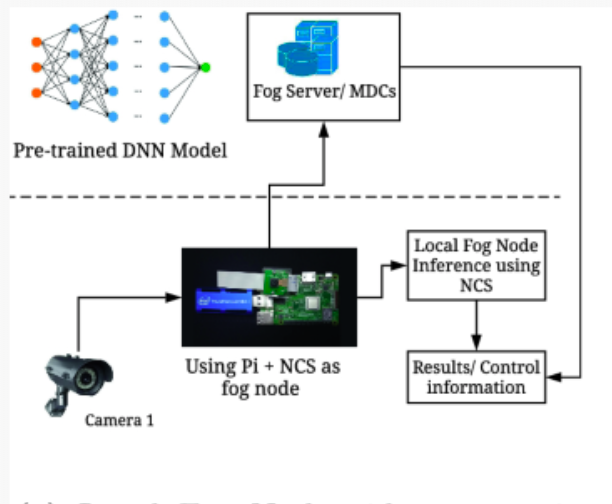
\includegraphics[width=7.0cm, height=7.0cm]{./2.png}
  \caption{the Local Fog Node using SSN}
  \label{natasha}
 \end{minipage}
  \begin{minipage}{.5\textwidth}
  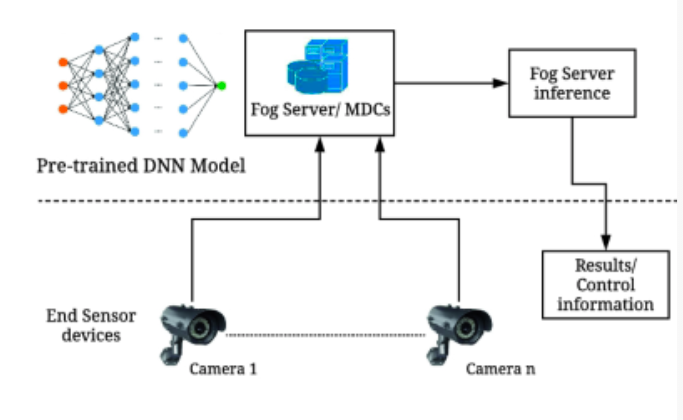
\includegraphics[width=7.0cm, height=7.0cm]{./3.png}
  \caption{Fog Server video processing using DNN}
  \label{natasha2}
 \end{minipage}
\end{figure}
\newpage
\item Sinqadu et al \cite{6} mentioned that using cloud-based architectures faces low latency when dealing with sensitive real-time applications; Therefore a new fog-based model for traffic surveillance was proposed. This model is based on three phases, inputting the IoT video streams, recognizing and tracking. Then, They used the ifogSim tool to simulate their approach using Fog Devices, Sensor, Actuator, Tuple class, and Application class. The results compared to cloud-based systems proved to be efficient in the average latency, energy consumption, data transfer rate, and more. This paper also proved that fog-based applications do better than cloud ones.

\item Santamaria et al \cite{Santamaria2019} mentioned that due to the large number of data collected by surveillance cameras, many challenges appeared in analyzing, storing, and retrieving data. In this chapter they are introducing the basics needs to build a framework for people's abnormal behaviors, after investigating the current techniques and technologies. Distributed architecture, Figure \ref{Santamaria}, was the main solution as it helps in enhancing the performance of the system. In addition, they mentioned the responsibility of each layer in the system, the possible computer vision techniques that can be used with their pros and cons as Neural networks, and the KNN model for Object detection and tracking.

\begin{figure}[!ht]
\centering
 \begin{minipage}{.5\textwidth}
  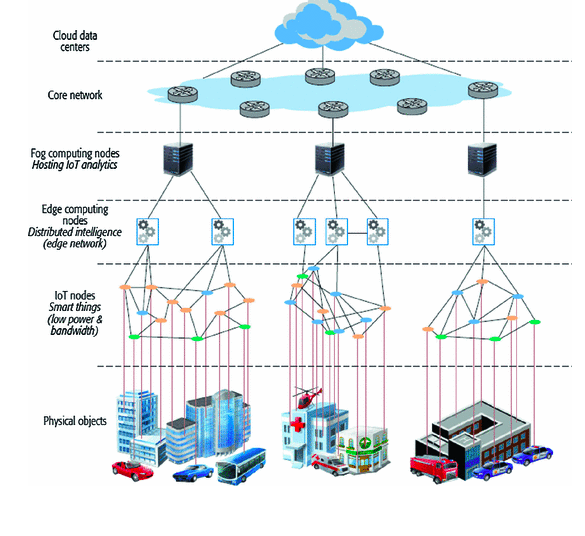
\includegraphics[width=10.0cm, height=10.0cm]{./4.png}
  \caption{the Distributed eccosystem in cloud domain}
  \label{Santamaria}
 \end{minipage}
\end{figure}

\item Ioannis Ledakis et al \cite{ledakis2018adaptive} aim to create a real-time surveillance system for smart cities. One of the challenges that faces the system is big data. The surveillance system utilized many cameras in 24/7 mode to cover the whole city. So, a massive amount of video and audio data is being generated and needs to be processed. The data must be transmitted from the IoT devices to the central unit for processing analysis. The authors found that this way will lead to late latency, in addition to the complexity found when other various types of data are placed. In this article, the authors merge the cyber foraging approach for unloading of calculation tasks to machines in the nearest place to the devices. The aim is to create a Fog-Edge based surveillance system that can handle such massive data and provide the system with real-time data processing analysis and decision-making. The result shows that the system acts with high performance and low latency. 
\newpage
\item Ning Chen et al \cite{chen2016dynamic} proposed a Fog-based traffic surveillance system to ensure security for the citizens and reduce the crime rate in smart cities. They use drones to monitor the vehicles on the whole road. Also, the system offers various tracking methods for detecting and tracking the suspicious vehicle with high accuracy. The proposed system aims to solve the high latency challenge caused by transferring the massive amount of data generated by the devices to the cloud. They utilized Fog computing to provide the system with real-time analysis for data processing efficiently and rapidly decision-taking in case of detecting a suspicious vehicle or any abnormal events. The proposed experiment result is encouraging. It shows that the system can handle multi-target effectively with high performance and low latency.

\item Jianguo Chen et al \cite{chen2019distributed} proposed a deep learning-based distributed intelligent video surveillance system and deploy it in edge computing. Due to the massive data generated from the IoT devices and massive network communication, the system aims to solve such challenges and provide real-time and accurate data analysis with low latency. Therefore, the proposed system will transfer the computing data from the central network to the edge network. The proposed approach shows that the system performs well and can handle such a huge video data and provide accurate and accelerated analysis. Moreover, it shows that edge computing provides the system with scalability and flexibility.

\item Baladoni et al\cite{7983190} proposed a video surveillance platform for smart cities, as shown in Figure \ref{arch}, that presents the following main features: Opening to different video acquiring technologies, Plug-and-play, Flexibility, and scalability with the number of transmitting and receiving devices. The proposed technology is achieved by using SAN and NAN prototypes, that are recognized according to the SDN/NFV standard paradigm by using general purpose x86-based hardware equipped with a software SDN switch and a virtualization environment, as shown in Figure \ref{Desc}.The proposed platform presents a lot of advantages like reduction of network traffic, low end to end latency, OpEx and CapEx reduction, scalability and platform add-ons.


\begin{figure}[!ht]
 \begin{minipage}{.5\textwidth}
  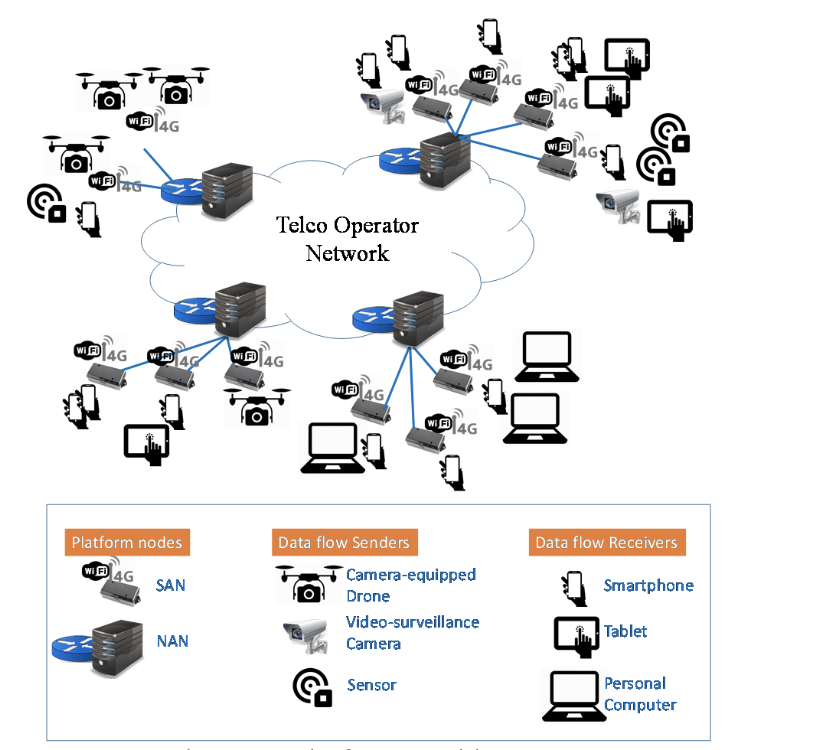
\includegraphics[width=7.0cm, height=7.0cm]{./10.png}
  \caption{Platfrom architecture}
  \label{arch}
 \end{minipage}
  \begin{minipage}{.5\textwidth}
  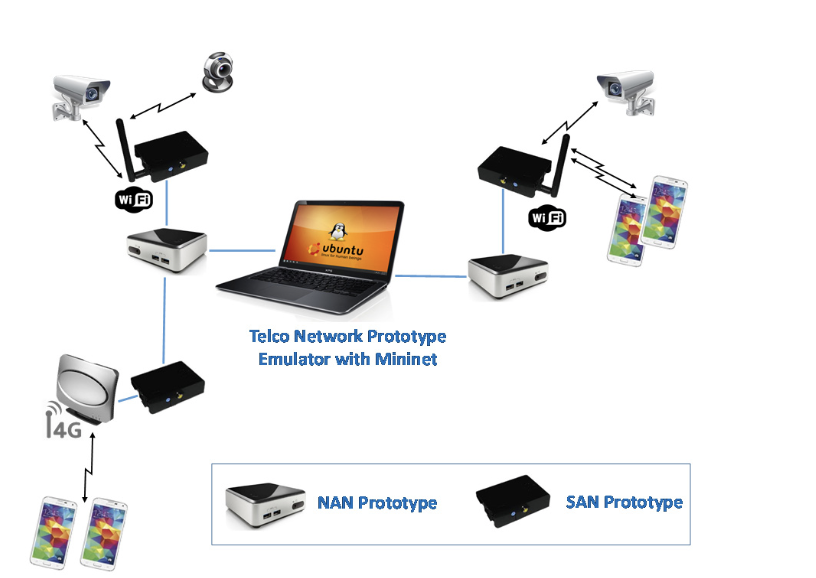
\includegraphics[width=7.0cm, height=7.0cm]{./11.png}
  \caption{Prototype description}
  \label{Desc}
 \end{minipage}
\end{figure}

\newpage

\item Xu et al\cite{9126126} presented a task offloading method for the video surveillance using edge computing, as shown in Figure \ref{edge}, that enables IoV to shorten the time cost, remain the load balance of edge nodes , and to maximize the privacy entropy. The authors presented a new algorithm design called TOM that solves multi-objective optimization problem by SPEA2(improving the strength Pareto evolutionary algorithm). Moreover, they implemented the normalization processing by TOPSIS (Technique for Order Preference by Similarity to Ideal Solution)and MCDM (Multiple Criteria Decision Making) methods. The final results shows that when the number of tasks is huge, TOM has stronger improvement on privacy protection than FFD algorithm which proofs that the experimental simulation performs efficient and trust.

\begin{figure}[!ht]
\centering
 \begin{minipage}{.5\textwidth}
  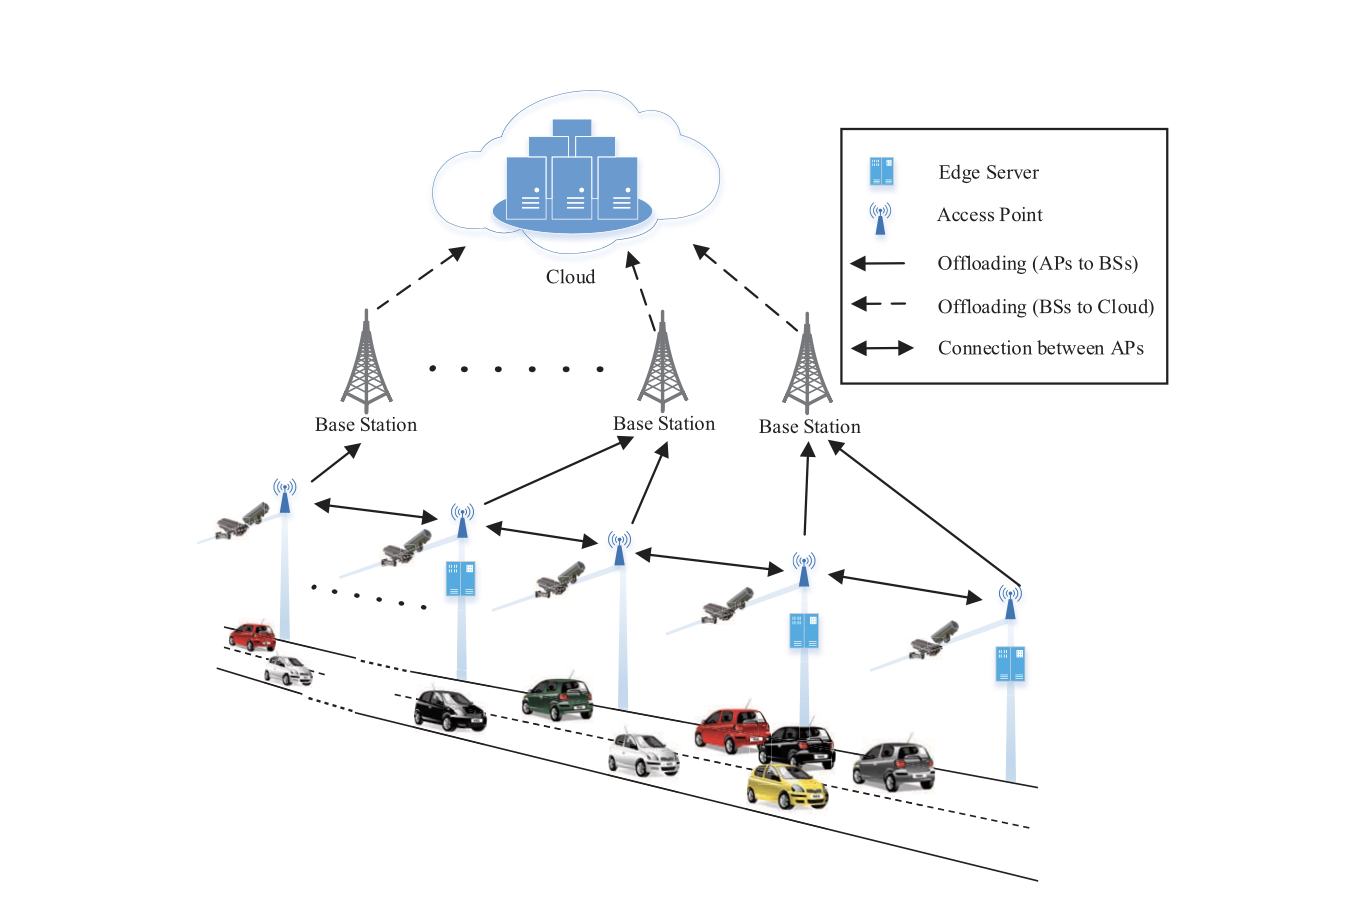
\includegraphics[width=10.0cm, height=10.0cm]{./12.png}
  \caption{A video surveillance architecture with the edge computing.}
  \label{edge}
 \end{minipage}
\end{figure}

\item  Sun et al \cite{8807184} mentioned that due to the large number of data collected by video surveillance, many challenges appear in the pre-processing stage. As a result, The authors proposed a video usefulness model,  (VU) model, for large scale video surveillance systems to detect failures in datasets in order to reduce the network bandwidth overload and improve the storage usage in the cloud, which is based on edge computing and cloud computing. In addition, efficiently and accurately analyzing useful video streams using suitable resources. Moreover, they mentioned ten different types of failures and categorized them into three main domains. They used a dataset from a realistic video surveillance system, that has approximately 4,433 IP cameras. In addition to 4,232 online cameras that contains different types of failures, to examine their proposed model. The types of failures they collected were conducted into two main groups: basic evaluation and scalability evaluation. The basic evolution is measured by two metrics, which are TP and TN. The results shows that their proposed model helps to reduce the bandwidth of the network and the amount of useless data that are stored in the cloud.

\end{itemize}
\subsection{Business Applications}
\begin{itemize}
\item  For the sake of demonstrating the smart city surveillance technology, Mark Witten \cite{witten_2020} discussed the case studies and the investigations proposed by David Murakami Wood, who is an investigator and a professor in surveillance studies at Queen’s University in Canada. First, the author states Wood’s  research observations on smart cities. The inspections show that surveillance systems have a huge role in the development of smart cities. However, one concern mentioned by professor Wood is the privacy of the cities’ citizens. Moreover, he argues that a good smart city is the one which a government has a role in, as technology companies work for their own favour rather than what’s best for the people.

\item The security world market website \cite{securityworldmarket.com} proposed an article about Operational Technology Systems (OTS), which is a Hong Kong company that offers monitoring systems to manage difficulties faced in smart cities. The company provides a mobile surveillance system that presents solutions for various barriers including illegal activity detection, operation management, safety measurement, etc. Moreover, it collects data effectively from urban areas to achieve efficient outcomes and fully satisfy its stakeholders. The mobile surveillance system, shown in Figure \ref{mobile}, is easy to install, provides continuous video recording, and supports numerous networking technologies such as WiFi, 4G, 3G, etc.
\begin{figure}[!ht]
\centering
 \begin{minipage}{.5\textwidth}
  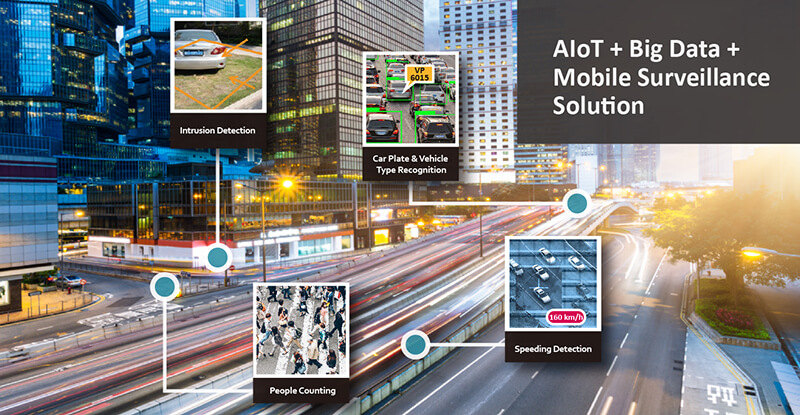
\includegraphics[width=12.0cm, height=8.0cm]{20190926-The-Intelligent-Traffic-Solution-Day-02.jpg}
  \caption{   OTS Mobile surveillance solution}
  \label{mobile}
 \end{minipage}
\end{figure}

\item Logipix Technical Development Ltd. \cite{logipix}, which is a privately held company established in 1996 in Budapest, Hungar, developed and manufactured intelligent video monitoring solutions specifically for large-scale projects and wide areas. They shared an article about the solutions they offer for safe smart cities. Furthermore, they highlighted their solutions as a scalable city-wide system that is designed to achieve traffic violation management and video surveillance tasks at the same time. Their goals are reducing the number of potential accidents and traffic jams using traffic violations detection algorithms, and providing a safe and secure system using an efficient surveillance large-scale system that secures the streets 24/7 with face recognition if possible.
\newpage
\item BT Busines \cite{BT} is a retail division of United Kingdom telecommunications company that provides many services, including IT services to businesses and a public sector in the UK and Ireland. They shared an article about smart cities and securing it, defining smart cities as intelligently connected cities in order to help the administrators make swift, decisions and helping them to fast respond to what’s going on and to prevent suspicious events before they happen. They helped many United Kingdom cities to turn to smart cities by the installation of cameras to help monitor traffics, give real-time alerts for trams, buses and etc, and many more. Finally, they gave easy steps to turn any city into a smart city by installing public WiFi, install cameras that can tell more in many cases and different situations, and controlling it.
\item Sara Wray \cite{Sara2020} focuses on the expansion and development of surveillance systems in smart cities all over the years. She mentioned that the global market for surveillance equipment in smart cities is at a significantly increased rate. Also, it is predictable for it to increase by a significant rate annually. Besides the fixed-video surveillance solutions, mobile surveillance solutions, as body-worn cameras and audio sensors, are getting popular. Moreover, she discussed the global trends for surveillance systems which state that china ranks first place in the geographical market. Also, India and Latin America are a fast-growing market. Moreover, she stated the importance of CCTV in monitoring to reduce crime rate effectively, it is also used in identifying suspects. Furthermore, she mentioned one of the most challenges that face the surveillance system in the public place which is privacy violation as a result of using a facial recognition feature.

\item Darwin smart city in Australia \cite{theconversation.com} installed a network that consists of new surveillance devices that cover all of the city to offer security and protection. The authors state that this web of “smart” lights, environmental sensors, and video cameras were designed to give the council more power to monitor and manage urban places. The council applied this system in the country to help them capture criminals, to encourage innovative solutions, increase safety in the country, and enhance community life. By now,  more countries in Australia are developing new police accurate schemes in surveillance systems to be applied in the future.

\item Technology is allowing cities to think quicker and act smarter \cite{sourcesecurity.com} by using  IOT and big data knowledge, as stated by Andrew Palmer.
For example, currently the local police councils and parking management systems are using surveillance technology to improve overcrowding and manage traffic flow. The author clarifies that cities that will be able to utilize surveillance data when considering any changes to their infrastructure will ultimately become the cities of tomorrow like Dubai.

\end{itemize}

\newpage
\section{What is new in the Proposed Project?}
Nowadays, with the expansion of video surveillance systems in public places, systems can expose the identity of people and transfer the private data to server-based video analysis, which make the data insecure  violates privacy rights. The proposed system will design Fog-Edge based surveillance system for smart cities. The system provides a real-time data processing analysis effectively and rapidly decision taking with high performance. Moreover, the system ensures privacy protection and secure citizen's data by balancing between the video analysis and unnecessary data that appear the user's identity in the video.

\section{Proof of concept}
Our system should proceed over several processes for it to perform effectively. As the first step is to model and simulate the system, we initiated the procedure by searching for an appropriate tool to use for building the system's architecture. As shown in Figure \ref{Sim}, iFogSim is a widely used simulation tool. Moreover, it is designed specifically for the modeling and simulation of fog computing, which makes it suitable to use in our project.
\begin{figure}[htp]
    \centering
    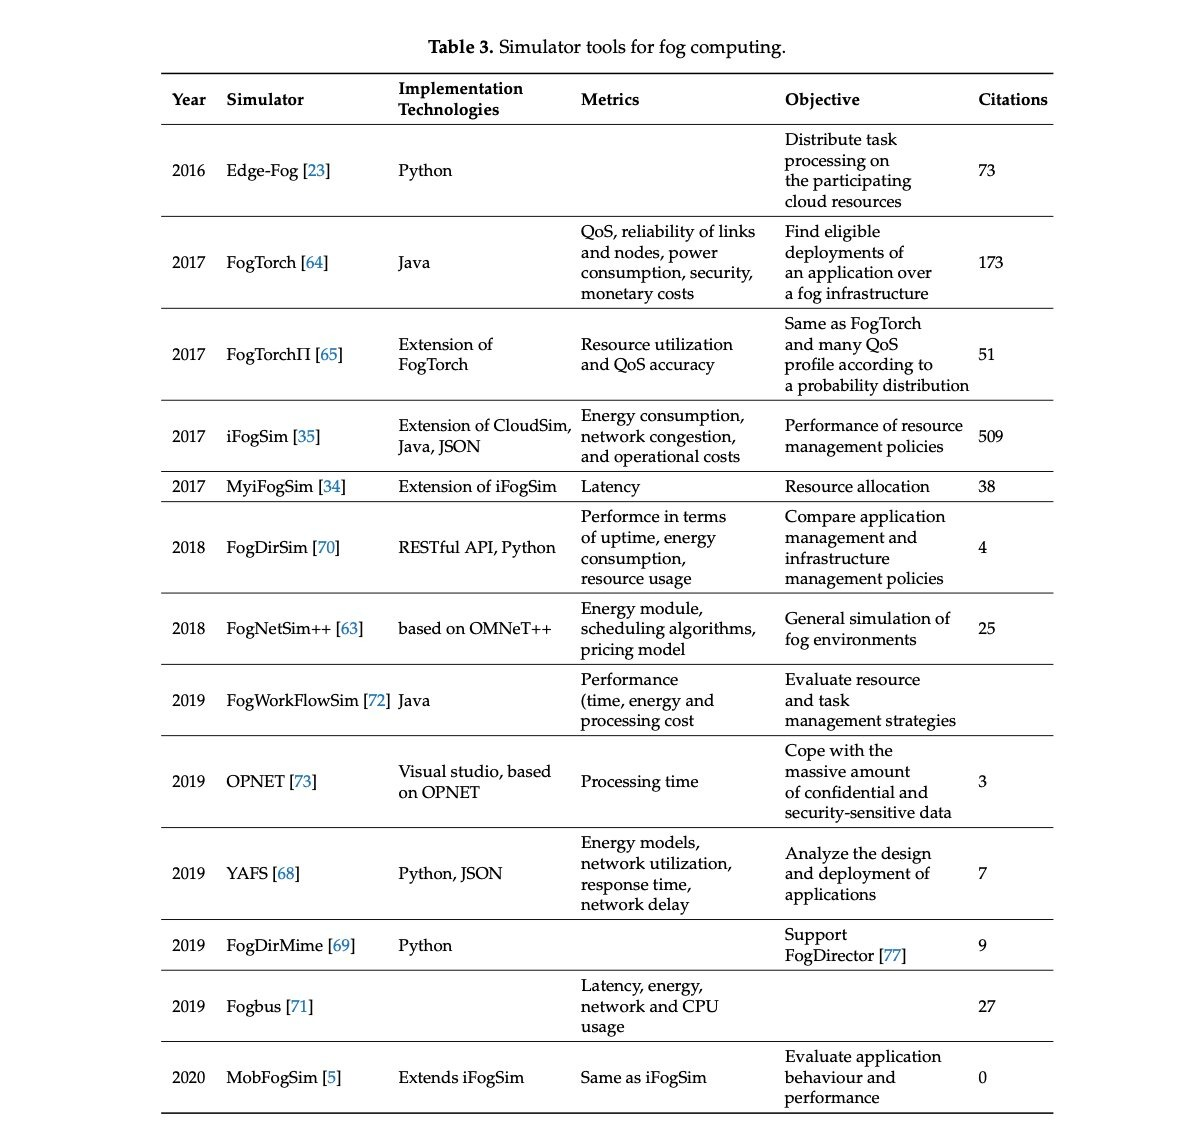
\includegraphics[width=13cm]{WhatsApp Image 2020-10-24 at 4.45.29 PM.jpeg}
    \caption{Simulator tools comparison}
    \label{Sim}
\end{figure}
\newpage
Additionally, we installed iFogSim and examined the features, packages, and the libraries introduced in it as a set up for our simulation process. As well as the components needed to perform simulation that are displayed in Figure \ref{ifogsim}: Physical Components, Logical Components, and Management Components.
\begin{figure}[htp]
    \centering
    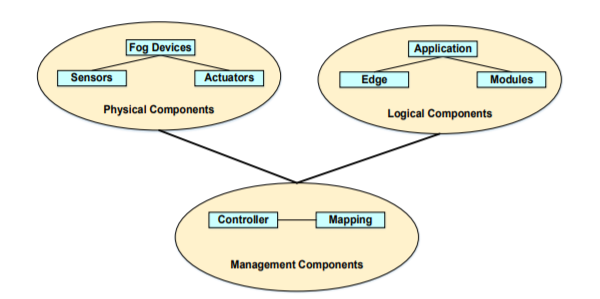
\includegraphics[width=20cm]{Screenshot (149).png}
    \caption{iFogSim simulation components}
    \label{ifogsim}
\end{figure}
\newline 
As Redowan Mahmud and Rajkumar Buyya \cite{mahmud2019modelling} illustrated, fog devices are required to be classified. After arranging them, we can then move to the logical components which are classified into three classes: AppEdge, AppModule, and AppLoop. These components are needed for the structure of the application. By means, the application module class identifies different modules within the application. Moreover, the Application edge connects modules with each other if any dependencies are visible. Lastly, the management components include the Controller and the Mapping class, which manage both the physical and logical components. The mapping class associates each accessible resource to the fog devices, according to the AppModule demands. Finally, the Controller collects all the results (cost, energy consumption, etc.).
\break
We inspected the DCNS.fog class in Figure \ref{fig} which contains
a case study for intelligent surveillance and examined the results presented in Figure \ref{fig1} .
\newpage
\begin{figure}[h]
   \centering
    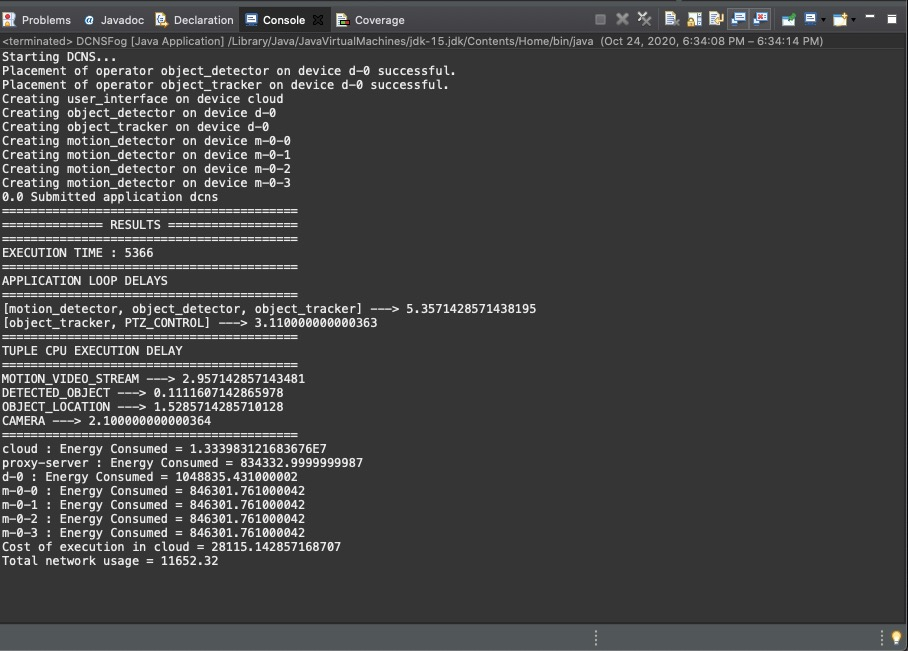
\includegraphics[width=10cm]{dcnsoutput.jpg}
    \caption{case study: intelligent surveillance output }
    \label{fig1}
    \newpage
    
     \centering
    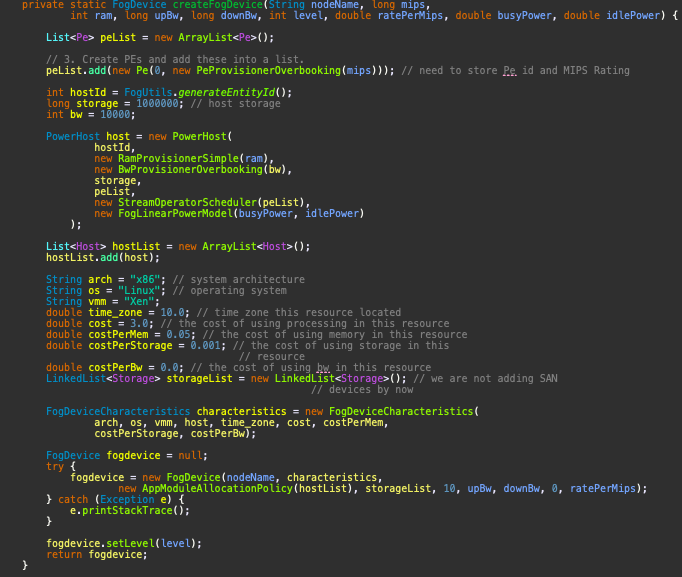
\includegraphics[width=10cm]{DCNSS.jpg}
    \caption{DCNS code }
    \label{fig}
\end{figure}

\newpage
In addition, we created a topology using the fog.GUI package, as shown in Figure\ref{fig:2}, as an initial step to developing an architectural design for our system, analyzing it, and starting up the implementation for our system.

\begin{figure}[h]
    \centering
    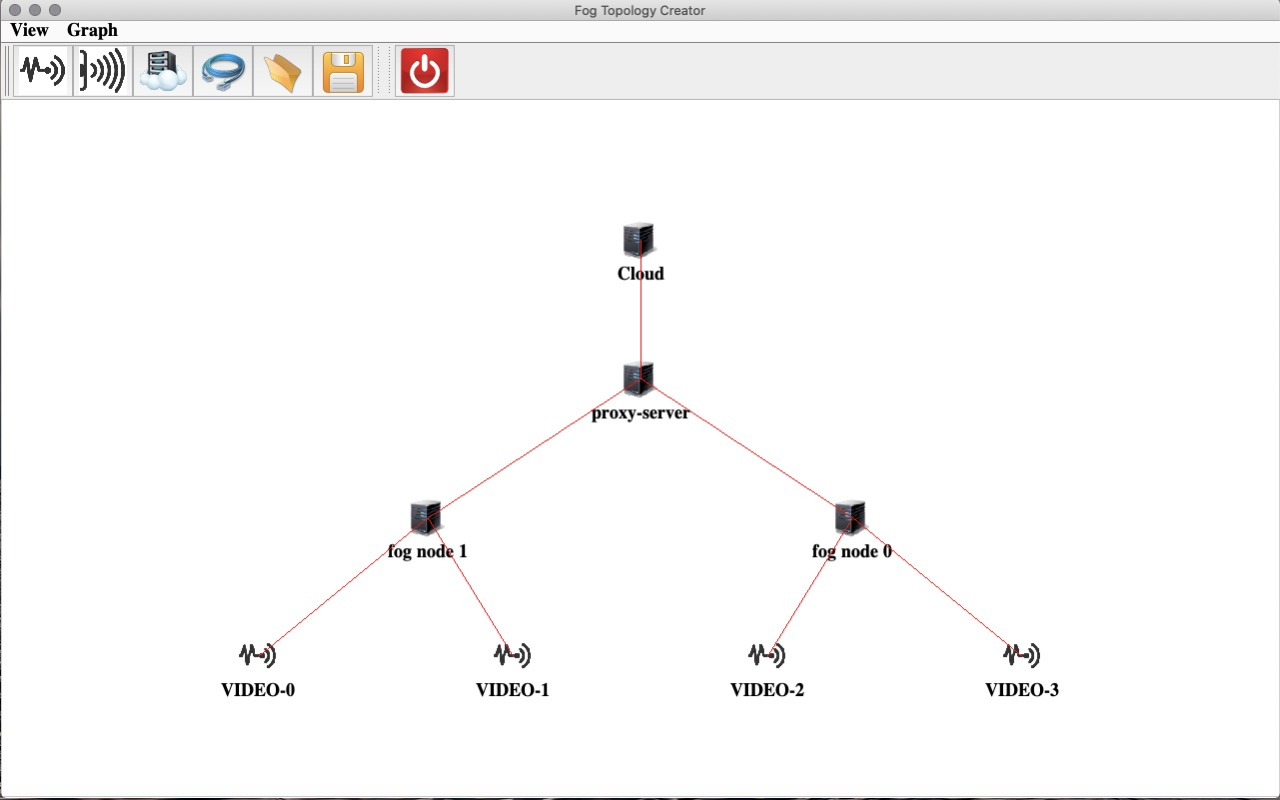
\includegraphics[width=10cm]{WhatsApp Image 2020-10-24 at 4.40.16 PM.jpeg}
    \caption{System topology }
    \label{fig:2}
\end{figure}

\subsection{Github}
\begin{figure}[h]
    \centering
    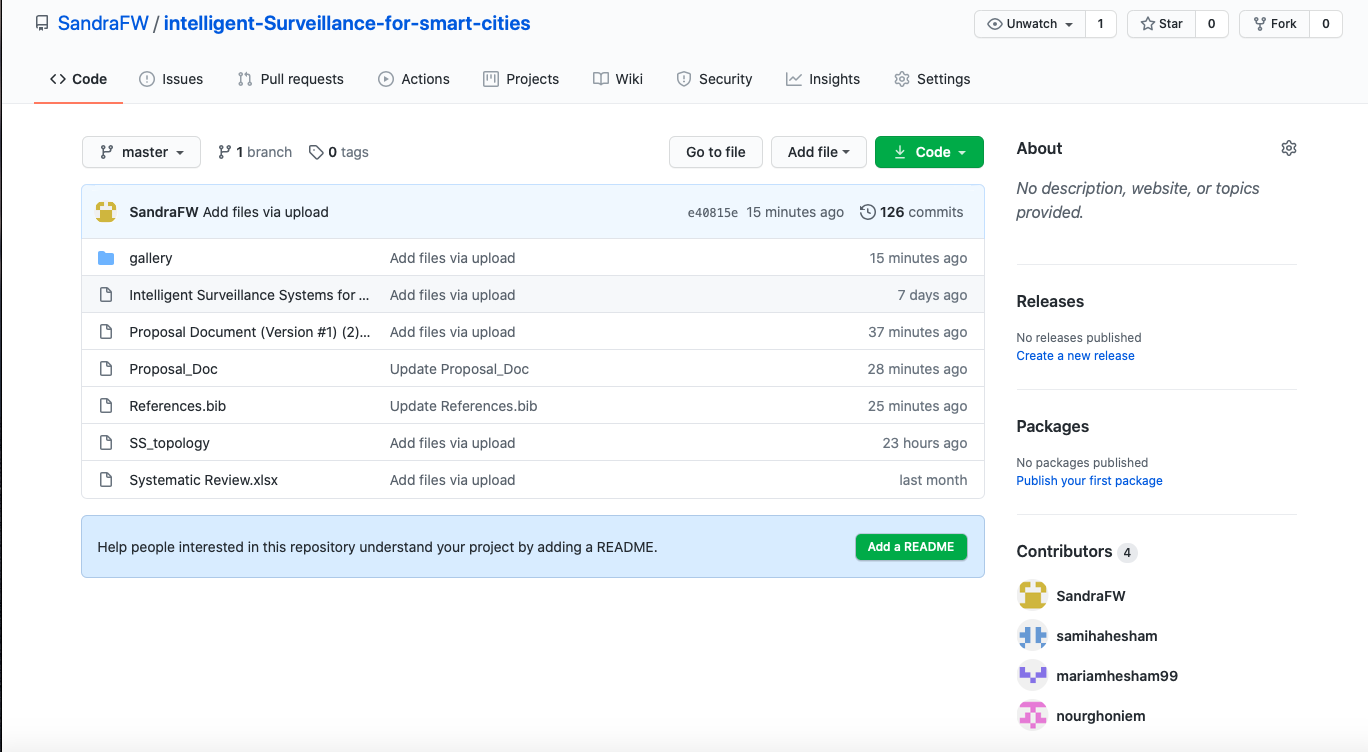
\includegraphics[width=12cm]{G1.png}
    \caption{Github Repository}
    \label{Repo}
\end{figure}

\begin{figure}[h]
    \centering
    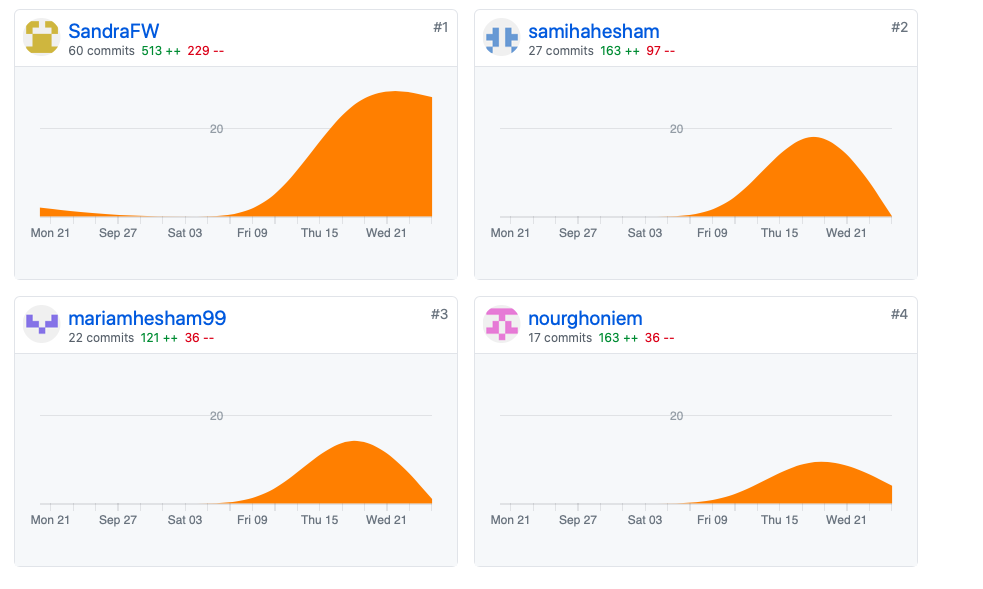
\includegraphics[width=13cm]{G2.png}
    \caption{Contribution }
    \label{Contrib}
\end{figure}

\newpage


\section{Project Management and Deliverables}
\subsection{Deliverables}
In order to reach our goal and obtain satisfactory results, we need to successfully achieve and deliver the fundamental elements of our system:

\begin{itemize}
\item System's architectural model
\item Algorithms for anomaly detection
\item Framework for video summarization
\item Privacy protection scheme    

\end{itemize}
First, the fog computing- based surveillance system architecture should be implemented using a simulation and modeling tool. Then, anomaly detection algorithms should be efficiently implemented to offer real-time data processing. Moreover, a framework should be developed for video summarization, in order to overcome the scalability challenge. In addition, privacy protection scheme will be presented for data security and to overcome privacy concerns in smart cities.

\hfill \break
\begin{table}[h]
    \centering
\begin{tabular}{|l|l|l|}
\hline 
\thead{Deliverables}    & \thead{Completion date}   \\ \hline
System Architecture & December 2020     \\ \hline
anomaly detection+ video summarization & February 2021 \\
\hline
Privacy protection scheme & April 2021 \\
\hline
\end{tabular}
\end{table}
\subsection{Management}
We used Trello, which is a web application that helps us manage our tasks and keep track of our progress. It includes the activities and work done by all the team members in each phase as shown in Figure \ref{trello} and Figure \ref{task}.
\newline
\textbf{Trello:}  {https://trello.com/b/7Z0ibwVz/graduation-project}   
\begin{figure}[htp]
    \centering
    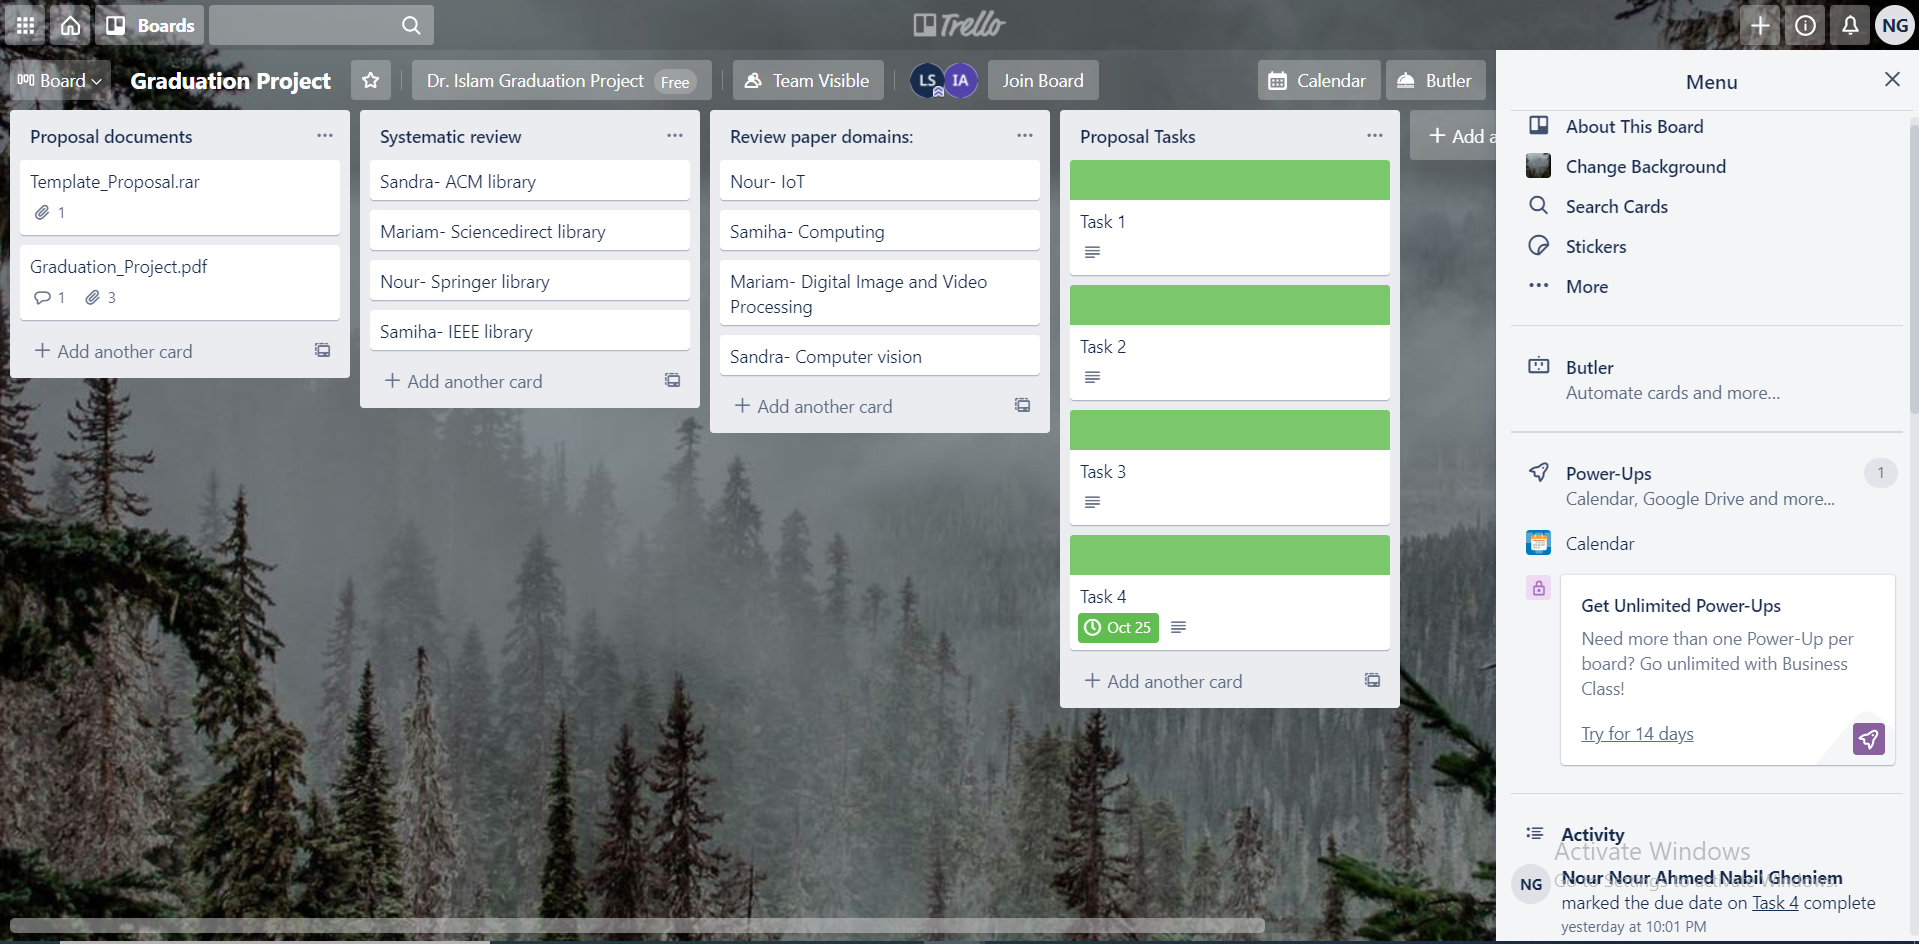
\includegraphics[width=14cm]{Screenshot (155).png}
    \caption{Trello: activity board}
    \label{trello}
\end{figure}
\begin{figure}[htp]
    \centering
    \includegraphics[width=9.2cm]{tasks.jpg}
    \caption{Trello: Proposal task cards}
    \label{task}
\end{figure}

\newpage
\section{Supportive Documents}
We have done a systematic review, as well as a review paper, which was sent to SSIC 2021(3rd International
Conference on Smart Systems: Innovations in Computing). we are waiting for their response.The paper is available on github.
    \begin{figure}[h]
    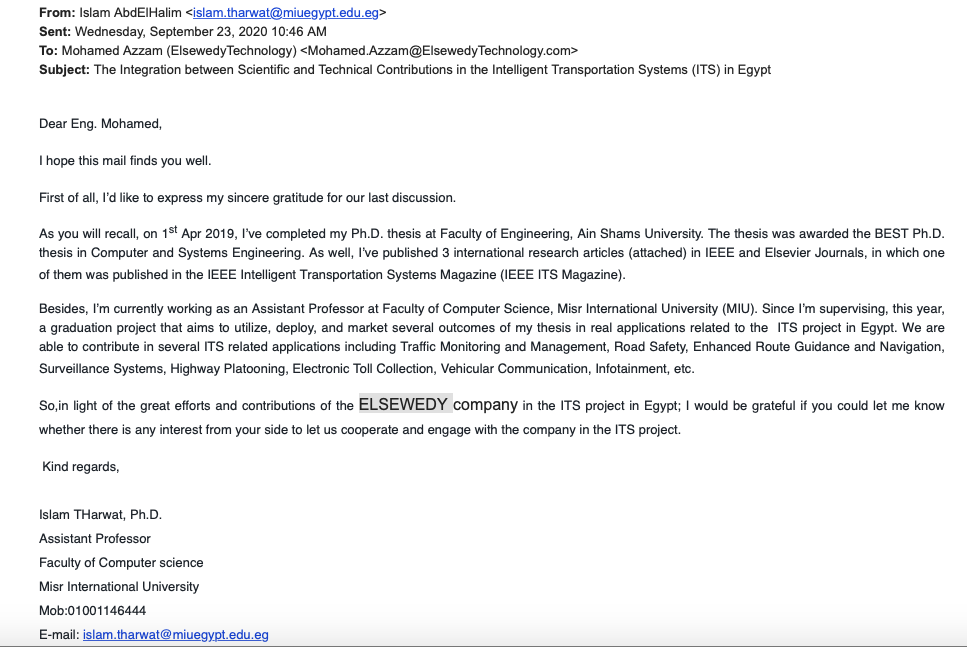
\includegraphics[width=13cm]{5.png}
    \caption{Contacting ELSEWEDY technology company}
    \end{figure}

    \begin{figure}[!h]
    
\includegraphics[width=13cm]{6.png}
    \caption{The company's response}
    \end{figure}
   \begin{figure}[htp]
    
\includegraphics[width=15cm]{8.png}
    \caption{Review Paper}
 \end{figure}
 \FloatBarrier
    \begin{figure}[htp]
    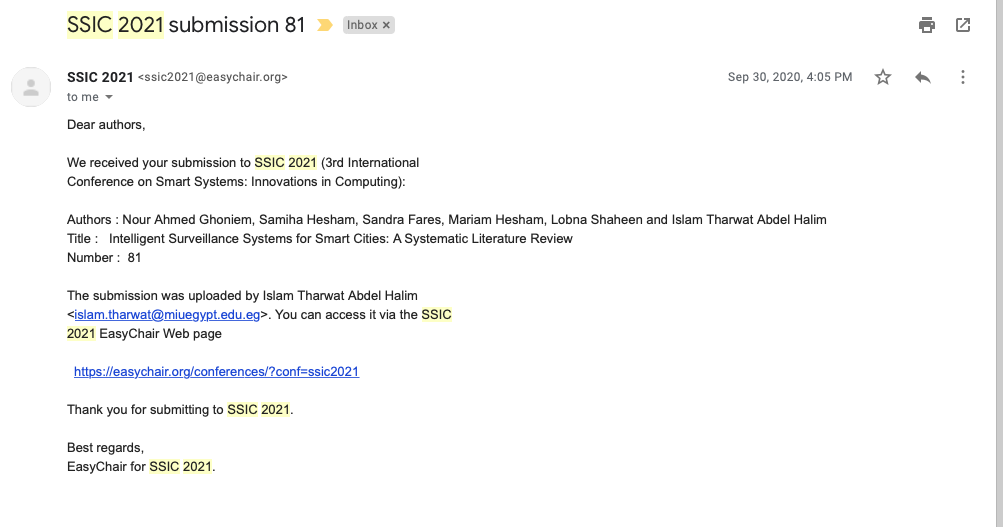
\includegraphics[width=15cm]{7.png}
    \caption{Submission email from SSIC 2021}

\end{figure}
\subsection{Tasks and Time Plan}

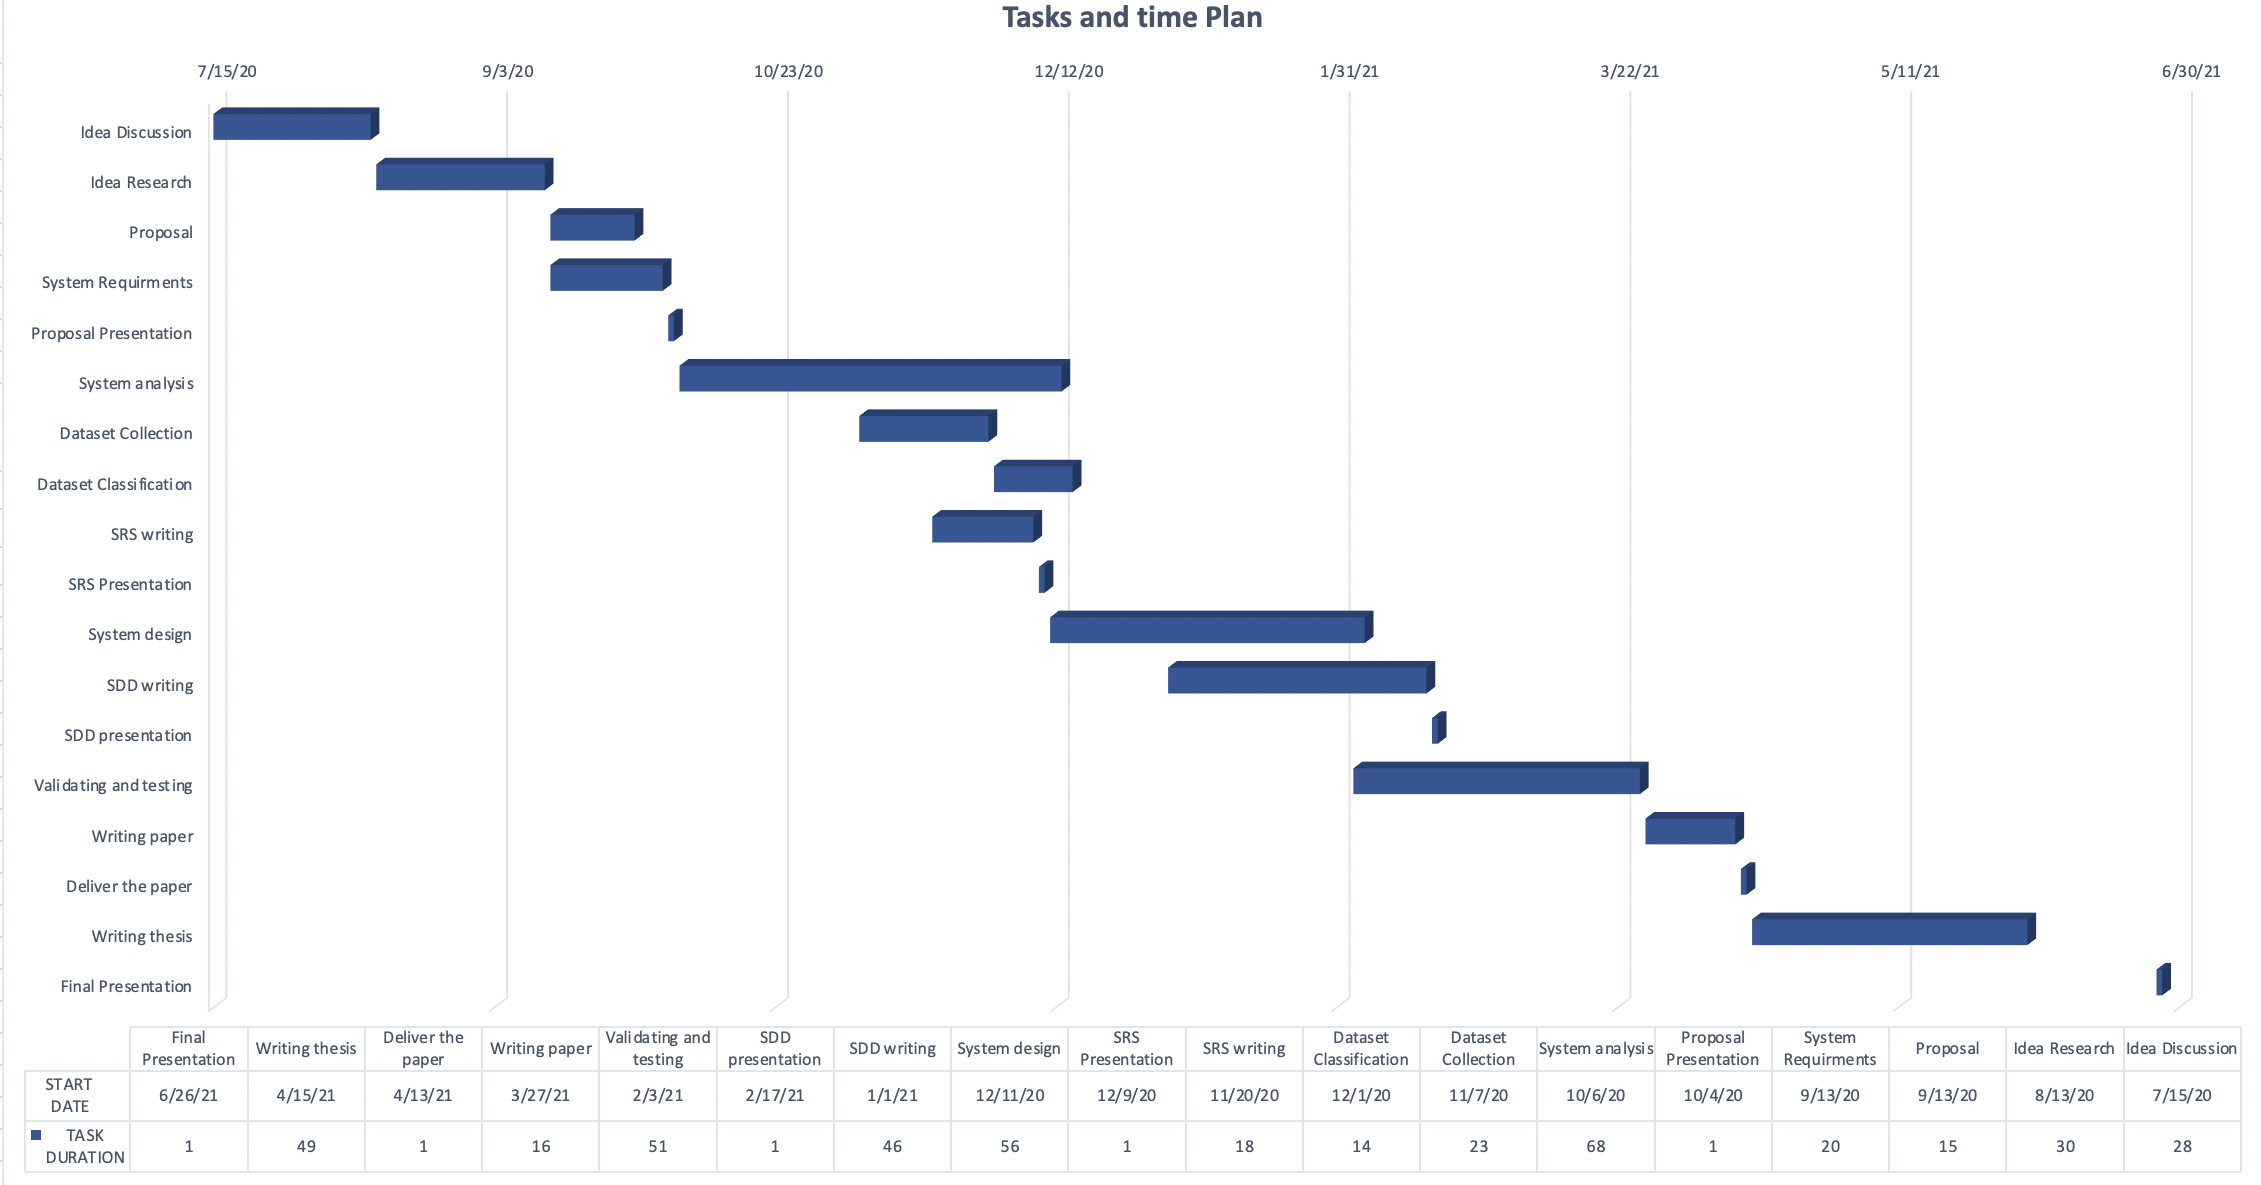
\includegraphics[width=1\textwidth]{./20.jpg}
\newline
\subsection{Budget and Resource Costs}
Article processing charges
\begin{itemize}
\item Articles publishing fees average: 2000\$.
\item Conference Registrations fees average: 330\$.
\end{itemize}

\section {References}
\nocite{*}
\printbibliography
\end{document}
